\documentclass{article}
\usepackage{final_project,times}
\newcommand{\comment}[1]{}
\usepackage[numbers]{natbib}
\usepackage{booktabs}
\usepackage{bbm}
\usepackage{float}
\usepackage{amsmath,amsthm,amsfonts,amssymb,amscd}
\usepackage{array}
%\usepackage{floatrow}
\usepackage{mathptmx}
\usepackage{alltt}
\usepackage{textcomp}
\newcolumntype{M}{>{$}c<{$}}
\usepackage{url}
\usepackage{graphicx}
\usepackage{subcaption}

%\documentstyle[nips12submit_09,times,art10]{article}


\title{Analyzing Market Cycles with Persistent Homology}


\author{
Aashiq Dheeraj, Christian Drappi \\
Math 412, Prof. John Harer \\
Department of Mathematics, Duke University
}

\newcommand{\fix}{\marginpar{FIX}}
\newcommand{\new}{\marginpar{NEW}}

\nipsfinalcopy

\begin{document}

\large

\maketitle

\begin{abstract}
<<<<<<< HEAD

\end{abstract}

\section{Introduction}

\section{Data}

\section{Analysis}

\section{Interpretation}

\section{Future Investigations}
=======
We examine stock price data from four major European indices between 1991 and 1998 using the machinery of Persistent Homology. First, we examine the topological structure of the stocks’ logarithmic returns. Secondly, we propose a method to predict future returns with homology, inspired by Elliott Wave Theory. Finally, we compare market behavior over different periods of time by clustering persistence diagrams.
\end{abstract}

\newpage

\section{Introduction}
Traders have different theories on price movements, derived from realms as diverse as stochastic processes and vedic astrology. Two of these include the Efficient Market Hypothesis and Elliot Wave Theory. The efficient market hypothesis holds that stock prices are a martingale, with an expected log return rate of 0 in the short run \cite{samuelson1965}. This view is popular among economists and mathematicians who can use this property to prove important results. However, many traders have had success using technical analysis-- the inference of future price movements from past patterns. The Elliot Wave Principle is one such technique, which suggests that the market oscillates between an optimistic, motive phase and a pessimistic, corrective phase at every time scale \cite{frost2005}. This cyclical motion is reminiscent of one-dimensional persistence. While we are sympathetic towards the efficient markets view, we decided to investigate the predictive power of cyclical motions in the market. 


\section{Data}
The data consists of prices of four major European indices – the DAX, SMI, CAC and FTSE – between 1991 and 1998. In mathematical theories of finance, price is not the quantity of interest; rather, financiers are more interested in the change in the logarithm of the price – the “log returns”. Therefore, we transformed our price data to log returns data. To do this, we divided the price from the $(t+1)$st time step by the price from the $t$th time step, and then computed its logarithm.

One convenience of using log returns is that they are additive. So, if we wished to understand topological structure in monthly log returns, we could simply add the log returns for each month, and compute persistence. 

\section{Methods}

\subsection{Persistent Homology over Log Returns}
We can compute persistence for the log returns data. The computation of the  0-dimensional diagram is similar to a general-purpose clustering algorithm. Persistent structure would suggest the existence of several distinct archetypes with characteristic return profiles. Returns on a given day could be characterized by one of these. The computation of the 1-dimensional persistence tells us about the existence of periodicity. 

We have too many points to blindly compute persistence over all length scales. We can generate the pairwise distance for 100,000 randomly selected days to get a sense for the characteristic length scales at which features might appear. We expect that most features should begin to appear before we connect each data point to a full half of the remaining data. We set the maximum edge length close to but below the median and proceed. The algorithm still takes an inordinate amount of time, so we can sample 200 points and compute persistence for these. This sampling is only done for exploratory analysis of the daily log-returns considered as a whole, and not for the chunked data considered below.

%% FIX THIS
\subsection{Wasserstein Distance}

We can separate the data into $n$-day chunks and compute the 1-dimensional persistence diagrams for each chunk, to characterize the cyclical behavior. The Wasserstein distance gives a metric for comparing persistence diagrams. Let $X$ and $Y$ be two persistence diagrams. A persistence diagram consists of a sequence of birth and death time pairs along with the infinitely many points on the diagonal where birth equals death . Let $\eta$ denote a perfect matcing between $X$ and $Y$, a bijection where points are matched up wherever possible and leftovers are sent to the closest point on the diagonal. Then the $q^{\text{th}}$ Wasserstein distance (WD)  is given by 
\[
W_q(X,Y) = \left[ \text{inf}_{\eta:X \rightarrow Y} \sum_{x \in X} || x  - \eta(x) ||^q_\infty \right]^{\frac{1}{q}}
\]

By computing the pairwise WD between chunks in the training set, we arrive at an $lfloor \frac{1833}{n} \rfloor$ -dimensional kernel, denoted $W_n$. We used Dmitriy Morozov’s Dionysus library for computation \cite{morozov2012}.

\subsection{Persistence of persistence diagrams}
Elliot Wave Theory maintains that cyclical structure in the markets is evident at every time scale. We can compute persistence on the set of persistence diagrams for an $n$-day partition of the data using $W_n$ as an explicit distance matrix. This gives a notion of structure among chunks considered as individual objects, elucidating the potential fractal structure of one-cycles.


\section{Interpretation}

\subsection{General persistence over log returns}
The resulting distribution is shown in the figure below. 
\begin{figure}
\begin{center}
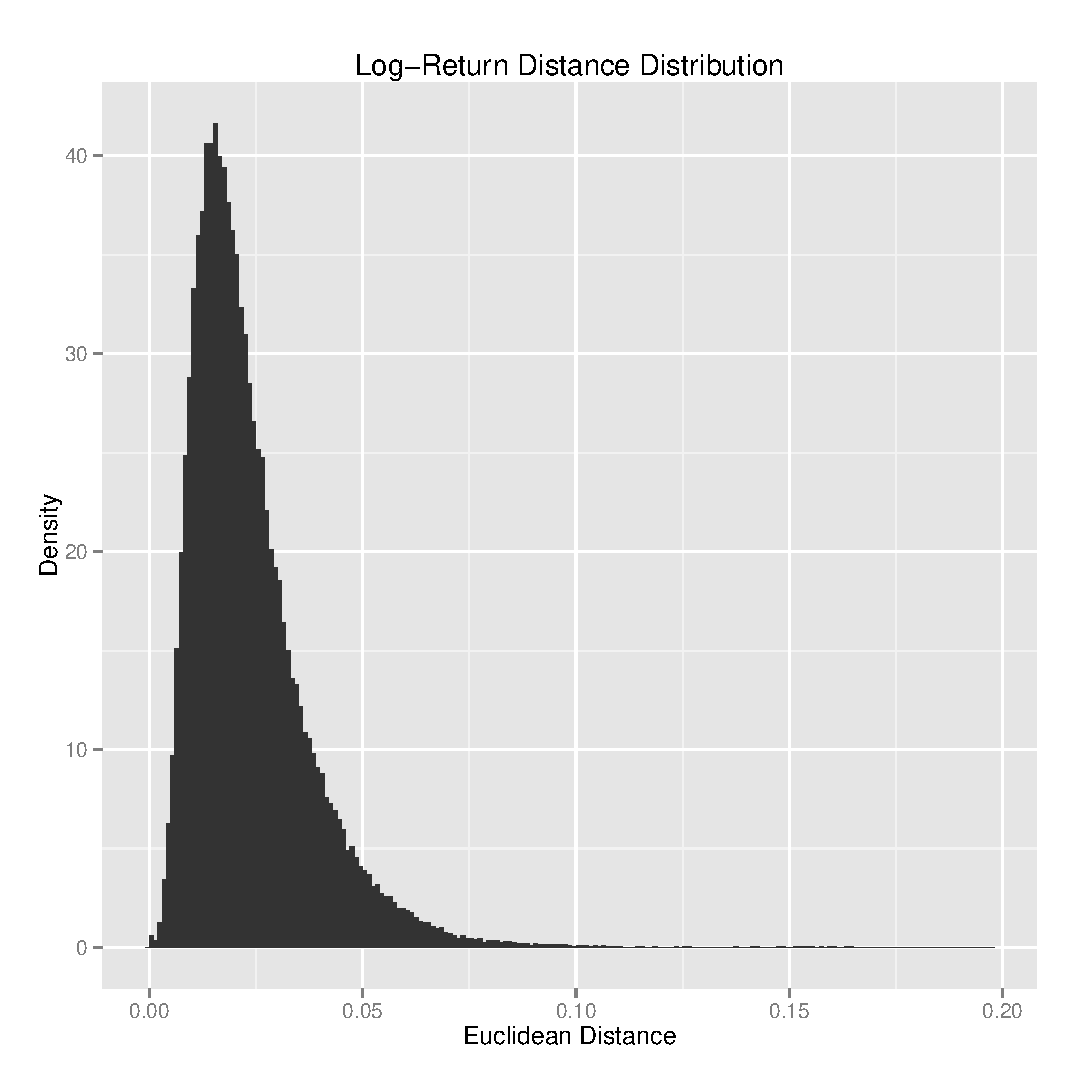
\includegraphics[width = 3.5 in, height = 3.5 in]{globplots/lr-dist}
\caption{The median is 0.02}
\label{lrdist}
\end{center}
\end{figure}



\begin{figure}
\centering
\begin{subfigure}[htbp]{0.45 \textwidth}
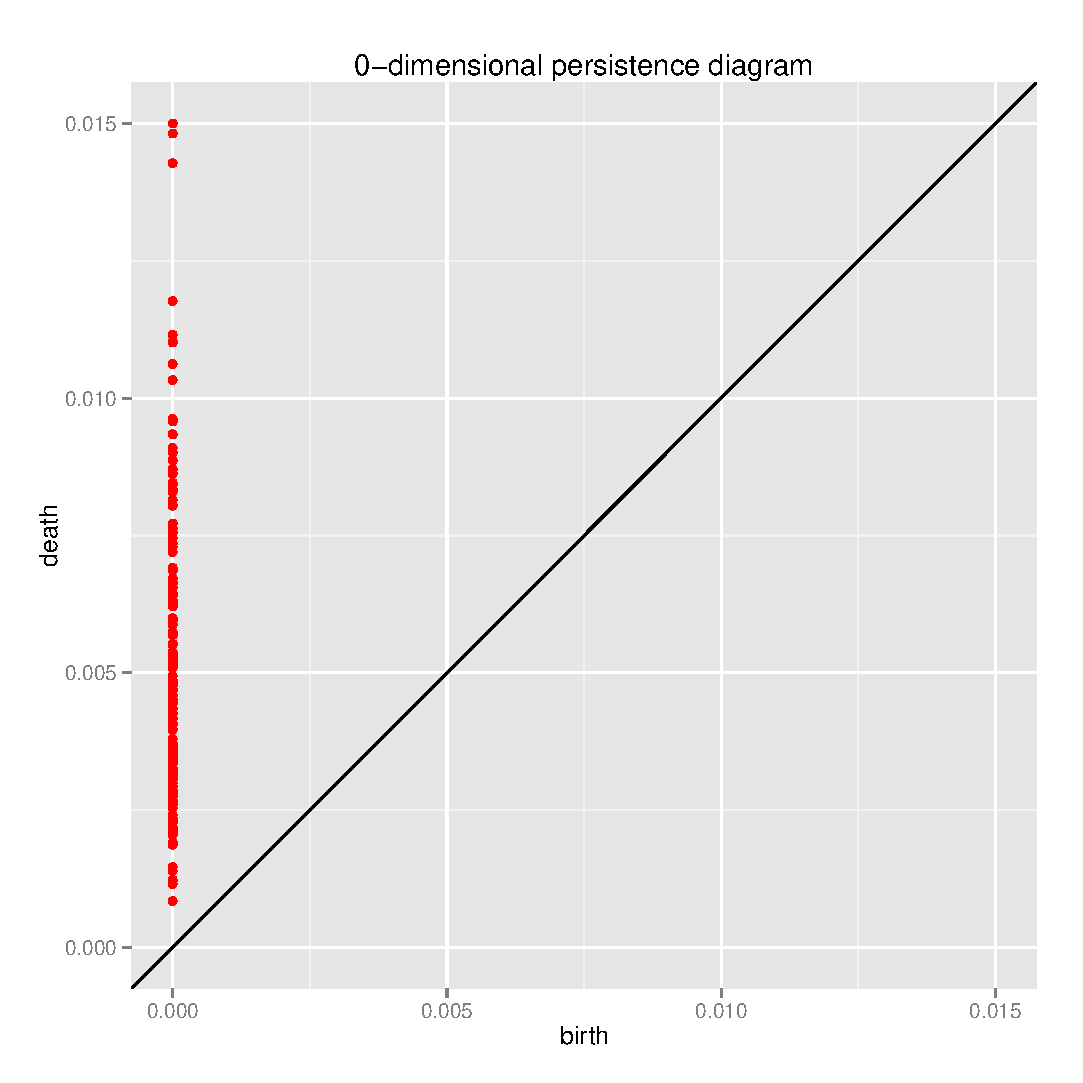
\includegraphics[width = \linewidth]{globplots/rlr-200-0-f15e-3}
\caption{We have a few clusters}
\label{lr0}
\end{subfigure}
~
\begin{subfigure}[htbp]{0.45 \textwidth}
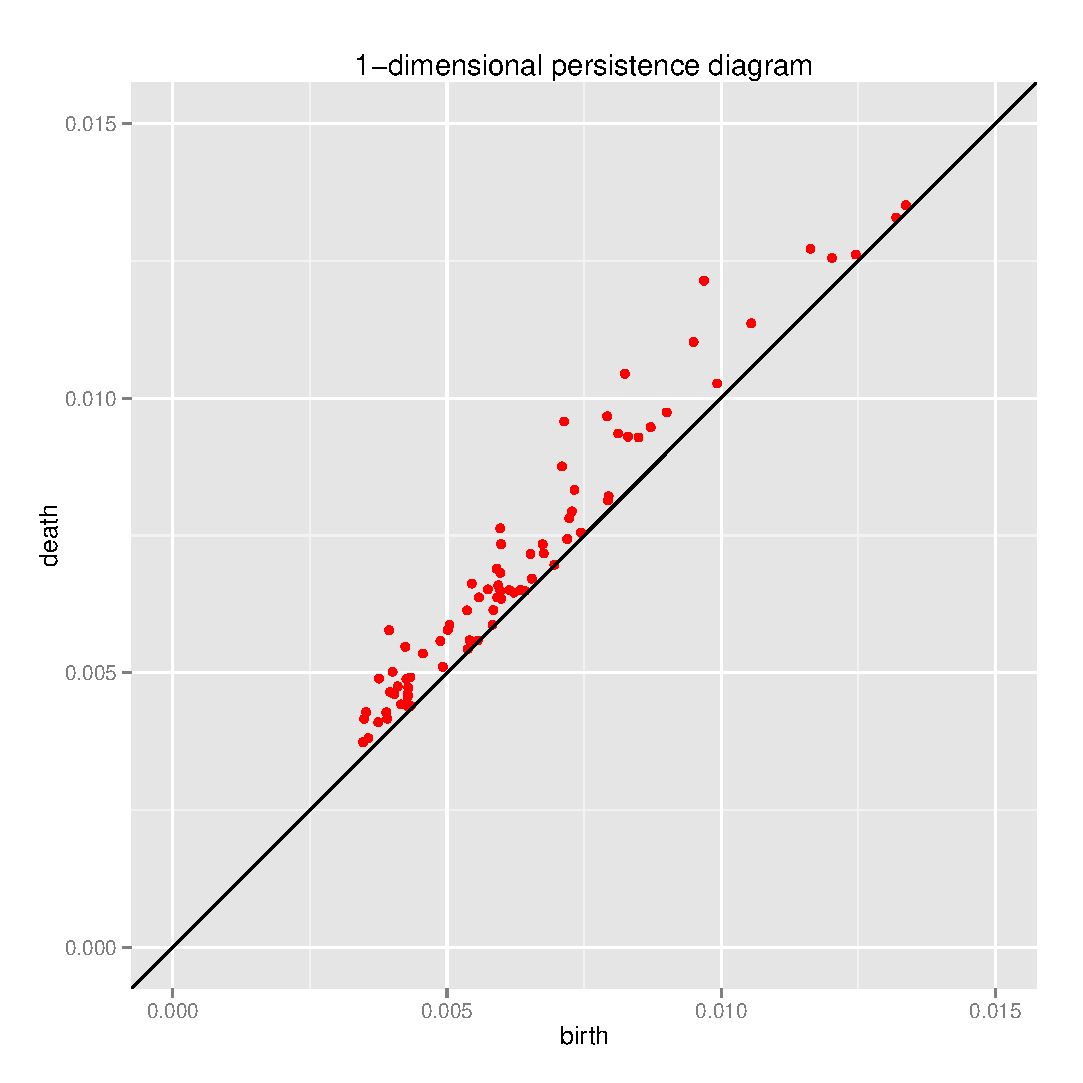
\includegraphics[width = \linewidth]{globplots/rlr-200-1-f15e-3}
\caption{There are no persistent 1-cycles}
\label{lr1}
\end{subfigure}
\label{lr}
\end{figure}



\subsection{Predicting Returns using Market Cycles}
Our method, chunk size = 30 0.08297711
Benchmark method, chunk size = 30 0.07266716
Our method, chunk size = 60, 0.1480877
Benchmark method, chunk size = 600.1218124
Our method, chunk size = 90 0.1176165
Benchmark method, chunk size = 90 0.1494282
Our method, chunk size = 100 0.1229456
Benchmark method, chunk size = 100 0.1583943


\subsection{Similarity over Time Scales}
Computing persistence between chunks resulted in trivial 0-D diagrams and slightly less trivial 1-D diagrams.

\begin{figure}
\centering
\begin{subfigure}[htbp]{0.45 \textwidth}
\includegraphics[width = \linewidth]{psqplots/p2-1-90}
\caption{$n = 30$}
\label{p2-1-30}
\end{subfigure}
~
\begin{subfigure}[htbp]{0.45 \textwidth}
\includegraphics[width = \linewidth]{psqplots/p2-1-60}
\caption{$n = 60$}
\label{p2-1-60}
\end{subfigure}

\begin{subfigure}[htbp]{0.45 \textwidth}
\includegraphics[width = \linewidth]{psqplots/p2-1-90}
\caption{$n = 90$}
\label{p2-1-90}
\end{subfigure}

\caption{1-D Persistence for Various Chunk Sizes}
\end{figure}

\section{Conclusion}

\section{Future Investigations}
\subsection{Kernel-Based Methods}
We have computed a kernel based on Wasserstein distance, and this can be used in a number of machine learning algorithms. Suppose we want to discriminate between winning, losing, and constant months. We can use our kernel to train a support vector machine, projecting our data into a higher-dimensional space where the three classes are linearly separable. Alternatively, we can employ PCA to reduce the dimensionality of the data. In this way, persistence diagrams might be characterized by  a few eigendiagrams.


\subsection{Options pricing}
In our investigation thus far, we have only considered this 4-dimensional data on European stock indices. The 4 indices are highly correlated, potentially accounting for the dearth of interesting structure. Alternatively, we might look at prices of options. American options give the holder the right but not the obligation to buy or sell a given security on or before a given date for a specified price. The value of an option is a function of the price of the underlying, the volatility, and the interest rate. These quantities are less correlated than the major  European indices, but are related in interesting ways in different market climates. Thus, we expect there to be more interesting topological structure.

\subsection{Explicit Time-Dependence}

\nocite{*}
\bibliography{final_project}
\bibliographystyle{ieeetr}


\end{document}




>>>>>>> 8fd379c06b249281c8275c4f41df58f16df0fa2b

